% created by Uwe Schadewald
% modified by Mathias Kuntze and Ahmet Uysal
% Add, handout to documentclass arguments for condensed pdf
\documentclass[presentation, 8pt, mathserif, t]{beamer} % , aspectratio=169
\usepackage[english]{babel}
\usepackage{pgf,graphicx}
\usepackage{amsmath, amssymb}
\usepackage[utf8]{inputenc}
\usepackage{lmodern}
\usepackage{palatino}
\usepackage{multimedia}
\usepackage{pgfpages} 
\usepackage{tikz}
\usepackage{datetime}
\pdfoptionpdfminorversion=5

\usepackage{caption}
\usepackage{subcaption}
% if else
\usepackage{ifthen}
% extend table options
\usepackage{tabularx} 
\usepackage{booktabs}
\usepackage{multicol}
\usepackage{multirow}
\usepackage{eso-pic}  % package to set background image
\usepackage[calc]{picture}

% Packages and stuff for ToDo list like itempoints
\usepackage{pifont}
\newcommand{\cmark}{\ding{51}}%
\newcommand{\xmark}{\ding{55}}%
\newcommand{\open}{$\square$}
\newcommand{\done}{\rlap{$\square$}{\raisebox{1pt}{\large\hspace{1.5pt}\cmark}}\hspace{-2.5pt}}
\newcommand{\wontfix}{\rlap{$\square$}{\raisebox{1pt}{\large\hspace{1.5pt}\xmark}}}
\newcommand{\notsure}{\rlap{$\square$}{\raisebox{0.8pt}{\large\hspace{1.5pt}\textbf{?}}}}



% side bar and footer
\setbeamertemplate{headline}{	
	\leavevmode
	\vspace{-4em}	
	\hbox{		
		\begin{beamercolorbox}[wd=0.85\paperwidth,ht=10ex,dp=8ex,center]{}%			
			% navigation with subsections as dots
			\hspace{3.5em}\insertnavigation{0.7\paperwidth}{\hskip0pt plus1fill} % add navigation in footer						
			% navigation with sections, no subsections
			% \insertsectionnavigationhorizontal{0.6\paperwidth}{\hskip0pt plus1fill}{} \\ % add navigation in footer}
			
		\end{beamercolorbox} 				
	}
	\vskip0pt
}


\setbeamertemplate{footline}{	
	\leavevmode
	\vspace{-3em}
	\hbox{
		\begin{beamercolorbox}[wd=.33\paperwidth,ht=2.25ex,dp=1ex,left]{author in head/foot}%
			\hspace{5em}
			\insertshortauthor
		\end{beamercolorbox}
		\begin{beamercolorbox}[wd=.33\paperwidth,ht=2.25ex,dp=1ex,center]{title in head/foot}%
			\insertshorttitle \ - \insertshortsubtitle
		\end{beamercolorbox}	
		\begin{beamercolorbox}[wd=0.30\paperwidth,ht=10ex,dp=8ex,right]{pagenumber in head/foot}			 	
			\insertframenumber % add page numbers
		\end{beamercolorbox}
	}			
	\vskip0pt
}



\setbeamertemplate{frametitle}{
	\ifthenelse{\equal{\insertframesubtitle}{}}{
		\vspace{0.6cm}
		\huge{\insertframetitle}
	}{
		\vspace{0.6cm}
		\small{\insertframetitle}\\
		\vspace{0.3cm}
		\huge{\insertframesubtitle}
    }		
}

	
% enumerate sections
\setbeamertemplate{section in head/foot}{\hfill\insertsectionheadnumber.~\insertsectionhead}
%\setbeamertemplate{section in head/foot shaded}{\color{structure!50}\hfill\insertsectionheadnumber.~\insertsectionhead}
\setbeamertemplate{section in toc}{\inserttocsectionnumber.~\inserttocsection}

%enumerate subsections
\setbeamertemplate{subsection in head/foot}{\hfill\insertsubsectionheadnumber.~\insertsubsectionhead}
\setbeamertemplate{subsection in head/foot shaded}{\color{structure!50}\hfill\insertsubsectionheadnumber.~\insertsubsectionhead}
%\setbeamertemplate{subsection in toc}[subsections numbered]
\setbeamertemplate{subsection in toc}{\vskip0.5em\leftskip=2em\inserttocsubsection\par}

%--------------------------Common------------------------------------------------------
\setbeamercovered{transparent} % make the beamer theme invisible
\usefonttheme{structurebold}
\beamertemplatenavigationsymbolsempty % set navigations helper function to off
\setbeamertemplate{bibliography item}[text]
\setbeamertemplate{note page}[plain]

%\setlist[itemize,1]{label={$\bullet$}} % \item are using bullets
\setbeamertemplate{itemize items}[circle]
	
	

	
% create a new command to show it on two screens
% I'm using dspdfviewer.
\newcommand{\setDualView} {
	\setbeameroption{show notes on second screen=right}
}

%\AtBeginSection[]{\subsection{}}
\newcommand{\addcite}[1]{%
	\AddToShipoutPictureFG*{%
		\AtPageLowerLeft{%
			\put(0.90\paperwidth,5em){											
				\tiny{
					\cite{#1} 
				}			
			}
		}
	}	
}

% insert a frame with references -> use bibtex
\newcommand{\insertReferenceFrame}[3]{%
	\section{#1}
	\begin{frame}[allowframebreaks]
		\frametitle{#1}
		\bibliographystyle{#2}
		\bibliography{#3}
	\end{frame}	
}

\AtBeginSection[]{\subsection{}}
	





\usepackage{../KU-Beamer-Template/style/koc} 
\usepackage{minted}
\usepackage{upquote}

\title{KOLT Python} 
\subtitle{Review 1: Connect Four} 
\newdate{date}{06}{03}{2019}
\date{\displaydate{date}}
\author{Ahmet Uysal}

\titlegraphic{
\includegraphics[scale=0.2]{../KU-Beamer-Template/style/images/logo_kolt.eps}}

\setbeamercovered{invisible} % transparent

\begin{document}
    \maketitle
    \frame{\frametitle{Agenda}\tableofcontents}

    \section{Variables \& I/O}

        \begin{frame}{Comments}
            \LARGE
            \inputminted[frame=single,framesep=2pt]{python3}{../Lecture1/code-examples/comments.py}
            Python will basically ignore comments, they are purely written \textbf{for humans}!
        \end{frame}

        \begin{frame}{Variables}
            \LARGE
            \begin{table}[]
                \resizebox{0.8\textwidth}{!}{
                \begin{tabular}{|l|l|l|}
                \hline
                \textcolor{koc}{\textbf{Type}} &\textcolor{koc}{\textbf{Explanation}} & \textcolor{koc}{\textbf{Examples}} \\ \hline
                \textbf{\texttt{int}}  & represent \textbf{integers} & 3, 4, 17, -10 \\ \hline 
                \textbf{\texttt{float}} & represent \textbf{real numbers} & 3.0, 1.11, -109.123123 \\ \hline
                \textbf{\texttt{bool}} & represent \textbf{boolean} truth values & \texttt{True}, \texttt{False} \\ \hline
                \textbf{\texttt{str}} & A sequence of characters. & \textquotesingle Hello\textquotesingle, \textquotesingle \textquotesingle, \textquotesingle 3\textquotesingle \\ \hline
                \textbf{\texttt{NoneType}}& special and has one value, None & \texttt{None} \\ \hline
                \end{tabular}}
            \end{table}
            \begin{itemize}
                \item How to create a variable?        
                \texttt{variable\_name = value}
                \item How about types?
                use \texttt{type()}
                \item Can a variable change type?
                \textbf{Yes!} Just assing a new value with any type.
                \item What if we if want to convert a value between types, i.e, \textquotesingle 2\textquotesingle $\to$ 2
            \end{itemize}
        \end{frame}

        \begin{frame}{Casting}
            \LARGE
            \begin{itemize}
                \item \texttt{int(\textquotesingle 2\textquotesingle)} $\to$ 2
                \item Any possible reasons for casting?
                -taking user input
                -reading numbers from a file?
                \item Can we cast every value to every type?
                \textbf{NO!} try \texttt{int(\textquotesingle hello\textquotesingle)}
            \end{itemize}
        \end{frame}

        \begin{frame}{Console I/O(Input/Output)}
            \huge
            \textbf{\texttt{print(*args, sep=\textquotesingle \ \textquotesingle, end=\textquotesingle \textbackslash n\textquotesingle )}}
            \begin{itemize}
                \LARGE
                \item Can take arbitrary number of arguments
                \item Separates elements with space by default
                \item Adds newline character \texttt{\textquotesingle \textbackslash n\textquotesingle} to end by default
            \end{itemize}
            \textbf{\texttt{input([prompt])}}
            \begin{itemize}
                \LARGE
                \item Prints the prompt to Console
                \item Program is paused until user enters something
                \item \textbf{returns an \texttt{str} object!} 
            \end{itemize}
        \end{frame}

    \section{Basic Operators}
        
        \begin{frame}{\texttt{bool} Operators}
            \LARGE
            How to represent logical operations in Python? (and, or, not)
            \begin{table}[]
                \resizebox{0.45\textwidth}{!}{
                \begin{tabular}{|c|c|c|c|c|}
                \hline
                \textcolor{koc}{\textbf{A}} &\textcolor{koc}{\textbf{B}} & \textcolor{koc}{\textbf{A or B}} & \textcolor{koc}{\textbf{A and B}} & \textcolor{koc}{\textbf{not A}}\\ \hline
                \textbf{\texttt{True}}  & \textbf{\texttt{True}}  & \textbf{\texttt{True}}  & \textbf{\texttt{True}} & \textbf{\texttt{False}} \\ \hline
                \textbf{\texttt{True}} & \textbf{\texttt{False}}  & \textbf{\texttt{True}} & \textbf{\texttt{False}} & \textbf{\texttt{False}} \\ \hline
                \textbf{\texttt{False}} & \textbf{\texttt{True}}  & \textbf{\texttt{True}} & \textbf{\texttt{False}} & \textbf{\texttt{True}} \\ \hline
                \textbf{\texttt{False}} & \textbf{\texttt{False}} & \textbf{\texttt{False}} & \textbf{\texttt{False}} & \textbf{\texttt{True}} \\ \hline
                \end{tabular}}
            \end{table}
            
            \begin{columns}
                \column{0.25\textwidth}
                    \begin{itemize}
                        \item \textbf{\texttt{and}}
                        \item \textbf{\texttt{or}}
                        \item \textbf{\texttt{not}}
                    \end{itemize}
                \column{0.75\textwidth}
                    \texttt{True or False and False} $\Rightarrow$ \textbf{\texttt{True}} \\
                    \Huge
                    \centering
                    \textbf{WHY?}
            \end{columns}
        \end{frame}

        \begin{frame}{Operator Precedence}
            \LARGE
            Logical operators are evaluated in this order:
            \begin{enumerate}
                \item \texttt{not}
                \item \texttt{and}
                \item \texttt{or}
            \end{enumerate}
            You can override this order with parentheses\\
            \texttt{(True or False) and False} $\Rightarrow$ \textbf{\texttt{False}} \\
        \end{frame}

        \begin{frame}{Short-Circuit Evaluation}
            \LARGE
            \texttt{X}: Any boolean value\\
            \texttt{True or X} $\Rightarrow$ \textbf{\texttt{True}}\\
            \texttt{False and X} $\Rightarrow$ \textbf{\texttt{False}}\\
            Python is smart enough to take advantage of this!
            \inputminted[frame=single,framesep=2pt]{python3}{../Lecture2/code-examples/short_circuit.py}
        \end{frame}

        \begin{frame}{Arithmetic Operators}
            \LARGE
            These operations are applicable on Numeric types: \texttt{int} and \texttt{float}
            \begin{columns}
               \begin{column}{0.35\textwidth}
                \vspace{-5mm}
                \begin{itemize}
                    \item \texttt{+}: Addition
                    \item \texttt{-}: Subtraction
                    \item \texttt{*}: Multiplication
                    \item \texttt{/}: Division
                    \item \texttt{//}: Floor(integer) Division
                    \item \texttt{\%}: Modulo
                    \item \texttt{**}: Power 
                \end{itemize}
               \end{column}
               
               \begin{column}{0.65\textwidth}
                \inputminted[frame=single,framesep=2pt]{python3}{../Lecture2/code-examples/numeric_operators.py}
               \end{column} 
            \end{columns}
        \end{frame}

        \begin{frame}{Comparison Operators}
            \LARGE
            \begin{columns}
                \begin{column}{0.4\textwidth}
                    \begin{itemize}
                        \item \texttt{<}: Strictly less than
                        \item \texttt{<=}: Less than or equal
                        \item \texttt{>}: Strictly greater than
                        \item \texttt{>=}: Greater than or equal
                        \item \texttt{==}: Equal
                        \item \texttt{!=}: Not equal
                    \end{itemize}
                \end{column}
                
                \begin{column}{0.6\textwidth}
                    \inputminted[frame=single,framesep=2pt]{python3}{../Lecture2/code-examples/comparison.py}
                \end{column}
            \end{columns}
        \end{frame}

        \begin{frame}{Chained Comparisons}
            \LARGE  
            \texttt{1 < 2 < 3} $\Rightarrow$ \textbf{\texttt{True}}\\
            You can chain arbitrarily many comparison operations together.\\
            $v_{i}$: variables/values, $op_{i}$: comparison operators\\
            \texttt{$v_{1}\ op_{1}\ v_{2}\ op_{2}\ v_{3}\ ...\ op_{n-1}\ v_{n}$} is equivalent to:\\
            \texttt{$v_{1}\ op_{1}\ v_{2}$ \textbf{and} $v_{2}\ op_{2}\ v_{3}$ \textbf{and} ...$v_{n-1}\ op_{n-1}\ v_{n}$}\\
            \vspace{-4mm}
            \inputminted[frame=single,framesep=2pt]{python3}{../Lecture2/code-examples/chained.py}
        \end{frame}

        \begin{frame}{Assignment Operators}
            \LARGE
            We have already seen \texttt{\textquotesingle=\textquotesingle}: \texttt{variable\_name = value}\\
            Frequently we will update variables' values based on their \textbf{old value}.\\
            \textbf{Ex:} Increment a number: \texttt{num = num + 1}\\
            Python has shorthand representations for these updates with arithmetic operators.\\
            \texttt{num += 1} is equivalent to \texttt{num = num + 1}\\
            \texttt{result *= 2} is equivalent to \texttt{result = result * 2}\\
        \end{frame}

        \begin{frame}{Assignment Operators}
            \LARGE
			\begin{table}[]
				\resizebox{0.7\textwidth}{!}{
				\begin{tabular}{|l|l|l|}
				\hline
				\textcolor{koc}{\textbf{Operator}} &\textcolor{koc}{\textbf{Usage}} & \textcolor{koc}{\textbf{Equivalent}} \\ \hline
				\textbf{\texttt{+=}} & \texttt{val += 3} & \texttt{val = val + 3} \\ \hline 
				\textbf{\texttt{-=}} & \texttt{val -= 3} & \texttt{val = val - 3} \\ \hline
				\textbf{\texttt{*=}} & \texttt{val *= 3} & \texttt{val = val * 3} \\ \hline
				\textbf{\texttt{/=}} & \texttt{val /= 3} & \texttt{val = val / 3} \\ \hline
                \textbf{\texttt{\%=}}& \texttt{val \%= 3} & \texttt{val = val \% 3} \\ \hline
                \textbf{\texttt{**=}} & \texttt{val **= 3} & \texttt{val = val ** 3} \\ \hline
				\textbf{\texttt{//=}} & \texttt{val //= 3} & \texttt{val = val // 3} \\ \hline
				\end{tabular}}
			\end{table}
        \end{frame}

    \section{Branching}

        \begin{frame}{Branching}
            \vspace{-3mm}
            \begin{columns}
                \column{0.5\textwidth}
                \inputminted[firstline=1, lastline=4, frame=single,framesep=2pt]{python3}{../Lecture2/code-examples/branching.py}
                \inputminted[firstline=6, lastline=13, frame=single,framesep=2pt]{python3}{../Lecture2/code-examples/branching.py}
                \column{0.5\textwidth}
                \inputminted[firstline=15, lastline=27, frame=single,framesep=2pt]{python3}{../Lecture2/code-examples/branching.py}
            \end{columns}
            \begin{itemize}
                \item \texttt{<condition>} has a \textbf{\texttt{bool}} value (\texttt{True} or \texttt{False})
                \item Which expressions will be evaluated in which conditions?
            \end{itemize}
        \end{frame}

    \section{Lists}
        \begin{frame}{Lists}
            \begin{itemize}
                \LARGE
                \item Group values together.
                \pause 
                 \texttt{my\_values = [1, \textquotesingle a\textquotesingle, None]}
                \pause
                \item You can think of each element as a variable, accessed by \textbf{indexing}
                \pause
                \item You can do everything you do to variables to list elements:
                \pause
                    \begin{itemize}
                        \Large
                        \item Assign new values: \texttt{my\_values[0] = 3}
                        \pause
                        \item Use shorthand assignment operators: \texttt{my\_values[1] += \textquotesingle bc\textquotesingle}
                        \pause
                        \item Learn their type: \texttt{type(my\_values[2]) \# => <class \textquotesingle NoneType\textquotesingle>}
                        \pause
                        \item Change their type: \texttt{my\_values[2] = True}
                        \pause
                        \item Compare their value: \texttt{if my\_values[0] == my\_values[1]: ...}
                    \end{itemize}
                \pause
                \item What happens when we call \texttt{my\_values[3] = 3}?
                \pause
                 \texttt{\# => \textbf{IndexError}}
            \end{itemize}
        \end{frame}

        \begin{frame}{List Indexing}
            \LARGE
            Access elements at a particular index
            \begin{columns}
               \begin{column}{0.5\textwidth}
                \vspace{-5mm}
                \begin{figure}[H]
                    \bigskip
                    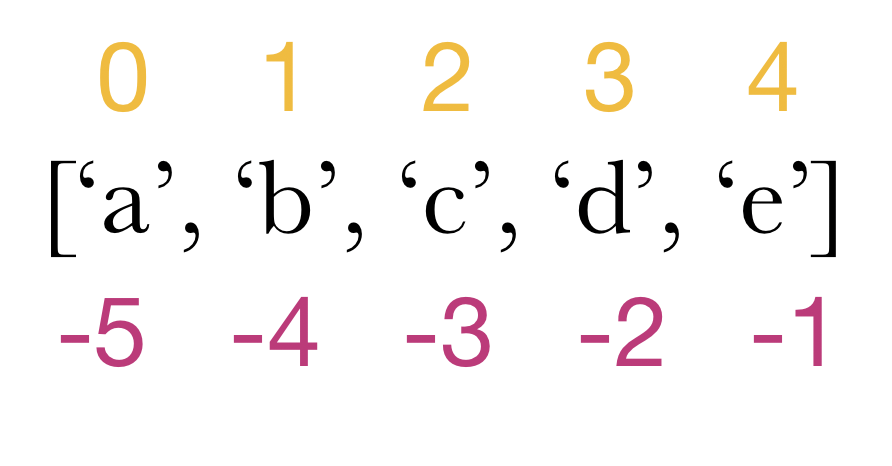
\includegraphics[width=70mm]{../Lecture3/code-examples/index.png}
                    \end{figure}    
               \end{column}
               \begin{column}{0.5\textwidth}
                \inputminted[frame=single,framesep=2pt, lastline=8]{python3}{../Lecture3/code-examples/index.py}
               \end{column} 
            \end{columns}
        \end{frame}

        \begin{frame}{List Slicing}
            \LARGE
            Access collection of elements by specifying \textbf{\texttt{[start:stop:step]}}\\
            \pause
            Gives a list, even when number of elements is not bigger than 1.
            \pause
            \normalsize
            \vspace{-2mm}
            \begin{columns}
                \begin{column}{0.5\textwidth}
                    \inputminted[frame=single,framesep=2pt,lastline=9]{python3}{code-examples/slicing.py}                        
                \end{column}                
                \begin{column}{0.5\textwidth}
                    \inputminted[frame=single,framesep=2pt,firstline=10]{python3}{code-examples/slicing.py}                                
                \end{column}
            \end{columns}
            \pause
            \vspace{2mm}
            \LARGE
            Slices with \texttt{step} = 1 are called \textbf{Basic Slice}.\\
            Slices with \texttt{step != 1} are called \textbf{Extended Slice}.
        \end{frame}


        \begin{frame}{List Mutation}
            \LARGE
            \pause
            \textbf{\texttt{list.append(x)}}: Append x to end of the sequence\\
            \pause
            \textbf{\texttt{list.insert(i, x)}}: Insert x to index i\\
            \pause
            \textbf{\texttt{list.pop(i=-1)}}: Remove and return element at index i\\
            \pause
            \textbf{\texttt{list.remove(x)}}: Remove first occurrence of x\\
            \pause
            \textbf{\texttt{list.extend(iterable)}}: Add all elements in iterable to end of list\\
            \pause
            \textbf{\texttt{list[i] = new\_value}}: Update value of index i with new value\\
            \pause
            \textbf{\texttt{list[basic\_slice] = iterable}}: Change elements in basic slice with elements in iterable, sizes can be different: \texttt{numbers[:] = []}\\
            \pause
            \textbf{\texttt{list[extended\_slice] = iterable}}: Change elements in extended slice with elements in iterable 1-1, sizes must be equal.\\
        \end{frame}

        \begin{frame}{Some Other List Operations}
            \LARGE
            \textbf{\texttt{in}} operator: Check whether an element is in list. \texttt{3 in numbers} $\Rightarrow$ \texttt{True}\\
            \textbf{\texttt{len(list)}}: Returns the length of list(and other collections).\\
            \textbf{\texttt{list.index(value, start=0, stop=len(list))}}: Return first index of value.\\
            \textbf{\texttt{list.count(value)}}: Count number of occurrences of value in list.\\
            \textbf{\texttt{list.reverse()}}: Reverse the list (in-place)\\
            \textbf{\texttt{list.sort()}}: Sort list elements (in-place)\\
            For more, type \texttt{help(list)} in your interactive interpreter.
        \end{frame}
    
    \section{Strings}
        \begin{frame}{Strings}
            \LARGE
            Special kind of \textbf{lists}!
            \pause
             \texttt{name = \textquotesingle Ahmet\textquotesingle\\}
            \pause
            You can do:
            \begin{itemize}
                \item Indexing: \texttt{name[2]} $\Rightarrow$ \textquotesingle m\textquotesingle
                \pause
                \item Slicing: \texttt{name[::-1]} $\Rightarrow$ \textquotesingle temhA\textquotesingle
                \pause
                \item Search by \texttt{in} operator: \texttt{\textquotesingle hm\textquotesingle in name} $\Rightarrow$ \texttt{True}
            \end{itemize}
            \pause
            You can not do:
            \begin{itemize}
                \item String mutation: \text{name[2]=\textquotesingle H\textquotesingle} $\Rightarrow$ \textbf{\texttt{TypeError}}
            \end{itemize}
            \pause
            Special functions about strings: \texttt{str.isnumeric(), str.capitalize(), str.format(...), str.find() ...}
        \end{frame}

    \section{Loops}
        \begin{frame}{Loops}
            \LARGE Do something for many elements or based on a condition.
            \begin{columns}
                \begin{column}{0.5\textwidth}
                    \inputminted[frame=single,framesep=2pt]{python3}{../Lecture3/code-examples/while1.py}
                    Similar to simple if blocks, but runs again and again until condition check fails.
                \end{column}
                \begin{column}{0.5\textwidth}
                    \inputminted[frame=single,framesep=2pt]{python3}{../Lecture3/code-examples/for1.py}
                    Iterable: collection of \textbf{ordered} elements.\\
                    What is next after this item?\\
                \end{column}
            \end{columns}
        \end{frame}

        \begin{frame}{For Loops}
            \LARGE
            What is next after this item?\\
            numbers[1] is after numbers[0]
            \pause
             \textbf{$\neq$ numbers[1] $>$ numbers[0]}\\
            \pause
            \textbf{Examples of iterables:}
            \pause
             lists,
            \pause
             strings,
            \pause
             ranges\\
            \pause
            \huge
            \\
            \textbf{Ranges}\\
            \LARGE
            \texttt{range(start, stop, step)}: creates a sequence of integers from start (inclusive) to stop (exclusive) by step.\\
            Can be \textbf{indexed} and \textbf{sliced}\\
            \texttt{len()} and \texttt{in} operator can be used
        \end{frame}

        \begin{frame}{For Loops}
            \inputminted[frame=single,framesep=2pt]{python3}{code-examples/for_loops.py}
        \end{frame}

        \begin{frame}{Break, Continue \& Pass}
            \begin{columns}
                \begin{column}{0.5\textwidth}
                    \textbf{Break}
                    terminates the closest for or while loop
                    \bigskip  
                    \inputminted[frame=single,framesep=2pt]{python3}{../Lecture3/code-examples/break1.py}
                    \inputminted[frame=single,framesep=2pt]{python3}{../Lecture3/code-examples/break2.py}
                \end{column}
                \begin{column}{0.5\textwidth}
                    \textbf{Continue}
                    continues with the next iteration of the loop
                    \bigskip  
                    \inputminted[frame=single,framesep=2pt]{python3}{../Lecture3/code-examples/continue1.py}
                    \inputminted[frame=single,framesep=2pt]{python3}{../Lecture3/code-examples/continue2.py}
                \end{column} 
            \end{columns}
        \end{frame}
        
        \begin{frame}{Break, Continue \& Pass}
            \textbf{Pass}
            does not have an effect
            \bigskip  
            \inputminted[frame=single,framesep=2pt]{python3}{../Lecture3/code-examples/pass.py}
            \begin{itemize}
                \item Loops, conditional statements, functions etc. cannot be empty 
                \item Use when you have to create one
            \end{itemize}
        \end{frame}

        \begin{frame}{For Else, While Else??}
            \texttt{else} in branching: executed when all of the conditions in upper \texttt{if}/\texttt{elif} blocks are False\\
            \pause
            \texttt{else} in loops: executed when loop is terminated \textbf{without} a \texttt{break} statement
            \pause
            \vspace{-3mm}
            \begin{columns}
                \begin{column}{0.52\textwidth}
                    \inputminted[frame=single,framesep=2pt]{python3}{code-examples/while_else.py}
                \end{column}
                \begin{column}{0.48\textwidth}
                    \inputminted[frame=single,framesep=2pt]{python3}{code-examples/for_else.py}
                \end{column}
            \end{columns}
        \end{frame}

    \section{Connect Four}

        \begin{frame}{Final Goal}
            \begin{center}                
               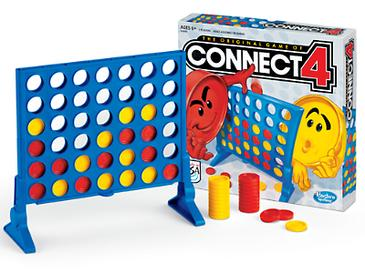
\includegraphics[height=0.75\textheight]{images/connect_4.jpg} 
            \end{center}
        \end{frame}

        \begin{frame}{Understanding the Board}
            \LARGE
            \inputminted[frame=single,framesep=2pt,firstline=12,lastline=18]{python3}{code-examples/connect_four.py}
            A nested \texttt{list}, each element stores a row (another \texttt{list}).\\
            First row, is stored at \texttt{board[0]}. How to iterate over rows?
        \end{frame}

        \begin{frame}{Printing the Board}
            \LARGE
            We need to print rows in reverse order, 0th row is printed at the bottom.\\
            We can use \textbf{slicing} to reverse, and a \texttt{for} loop to iterate.\\
            \texttt{\textbf{for} row \textbf{in} board[::-1]:}\\
            \\How can we print one row?
            \begin{itemize}
                \item Option 1: Iterate over all squares and print them one by one
                \item Option 2: Combine squares to one string and then print
                \item Hint: Check how \texttt{str.join()} works, can we use \texttt{\textquotesingle \ \textquotesingle.join(row)}?
            \end{itemize}
        \end{frame}

        \begin{frame}{Validating User Input}
            \LARGE
            What happens if players enter an invalid input?
            \begin{itemize}
                \item Enters his name instead of column no: Error when casting
                \item Enters \textquotesingle *\textquotesingle\ as symbol: Our logic is broken
            \end{itemize}
            How can we validate user input?
            \begin{itemize}
                \item Using \texttt{if} blocks? What if user enters another invalid input again?
                \item We need \textbf{loops}!
            \end{itemize}
        \end{frame}

        \begin{frame}{Validating User Input}
            \vspace{-2mm}
            \inputminted[frame=single,framesep=2pt]{python3}{code-examples/valid_input.py}
            \begin{itemize}
                \item If conditions are independent, create a single condition using logical operators
                \item Example: A symbol with length one, that is not \textquotesingle * \textquotesingle  and unused.
                \item \texttt{len(symbol) == 1 and symbol != \textquotesingle *\textquotesingle and symbol not in player\_pieces}
                \item What happens if conditions are dependant, for example get a non-full column no.
                \item It needs to be a valid number in the range 0-6, and the column shouldn't be full.
                \item We need number to be valid to check whether column is full.
            \end{itemize}
        \end{frame}

        \begin{frame}{Understanding the Game Flow}
            \LARGE
            \inputminted[frame=single,framesep=2pt,firstline=35,lastline=35]{python3}{code-examples/connect_four.py}
            What can we do with \texttt{move\_counter}?
            \begin{itemize}
                \item Understand whose turn it is:\\
                \texttt{print(\textquotesingle Turn is on \{\}\textquotesingle.format(players[move\_counter\%2]))}
                \item Understand which piece will be added:\\
                \texttt{player\_piece = player\_pieces[move\_counter\%len(players)]                }
                \item Understand how many moves game lasted.\\
                \texttt{move\_counter + 1}, why + 1?
            \end{itemize}
        \end{frame}

        \begin{frame}{Adding New Pieces to Board}
            \LARGE
            \begin{columns}
                \begin{column}{0.5\textwidth}
                    Assume we have the board below, turn is on yellow pieces, and user entered column 3.\\
                    \bigskip
                    \centering
                    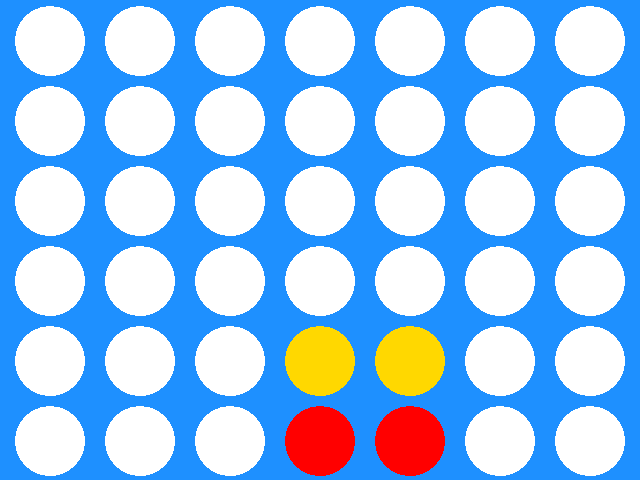
\includegraphics[width=0.6\textwidth]{images/connect_four_board.png}
                \end{column}
                \pause
                \begin{column}{0.5\textwidth}
                    Where should we add the new piece?\\
                    \pause
                    \bigskip
                    \centering
                    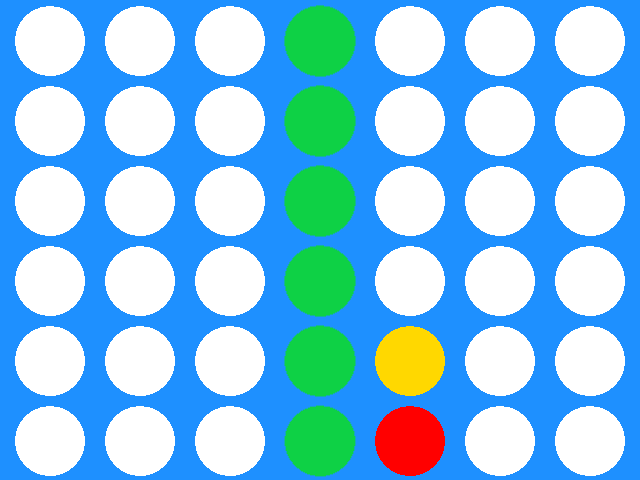
\includegraphics[width=0.6\textwidth]{images/connect_four_board_1.png}\\
                    To first \textbf{empty} square in that column
                \end{column}
            \end{columns}
        \end{frame}

        \begin{frame}{Finding the Empty Square}
            \LARGE
            How can we do that?
            \pause
             Iterate over columns
            \pause
            , but how?\\
            \pause
            Our representation of board is a list that contains rows\\
            We need to go over all rows to check the square in column 3\\
            Iterate over rows as we did before?\\
            \pause
            \inputminted[frame=single,framesep=2pt,lastline=4]{python3}{code-examples/finding_square.py}
        \end{frame}

        \begin{frame}{Finding the Empty Square}
            \Large
            \inputminted[frame=single,framesep=2pt,firstline=6]{python3}{code-examples/finding_square.py}
        \end{frame}

        \begin{frame}{Adding New Pieces to Board}
            \LARGE
            We found the square and added it to board
            \begin{center}
                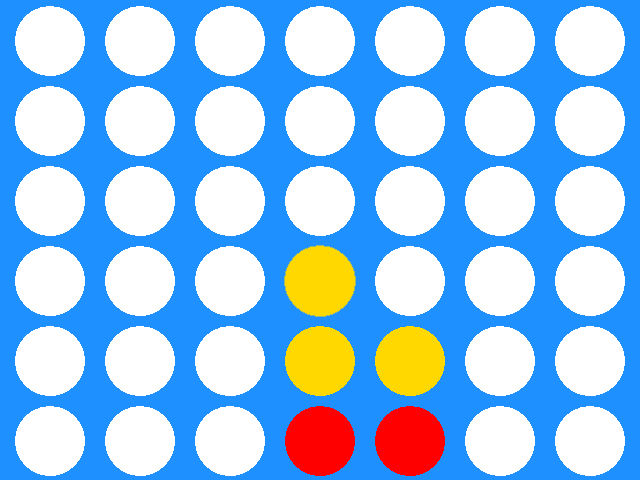
\includegraphics[height=0.6\textheight]{images/connect_four_board_2.png}\\
            \end{center}
            \vspace{-2mm}
            How to check whether the game ended or not?
        \end{frame}

        \begin{frame}{Check for Four Connected Pieces}
            \huge
            Before we start, some observations:
            \pause
            \begin{itemize}
                \item Yellow played the move, if game is ended winner is yellow pieces.
                \pause
                \item We can only check for yellow pieces since red cannot win in this move.
                \pause
                \item We don't have to check everywhere of board, we can be smarter. HOW?
            \end{itemize}
        \end{frame}

        \begin{frame}{Check for Four Connected Pieces}
            \LARGE
            We know new piece is added to row:2, column:3\\
            \begin{columns}
                \begin{column}{0.5\textwidth}
                    Check the row\\
                    \centering
                    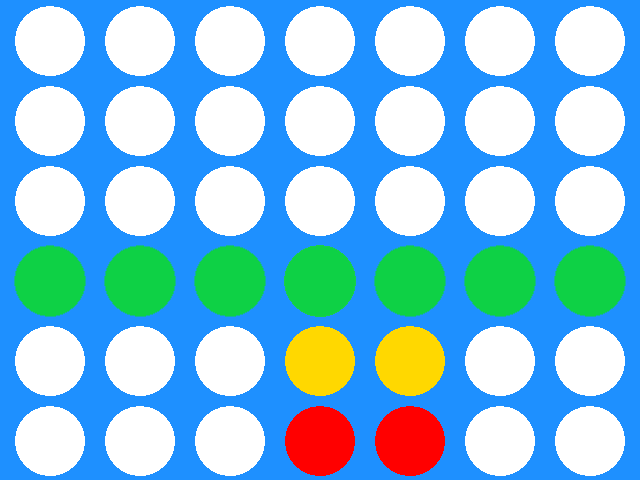
\includegraphics[width=0.6\textwidth]{images/connect_four_board_3.png}
                \end{column}
                \pause
                \begin{column}{0.5\textwidth}
                    Check the column\\
                    \centering
                    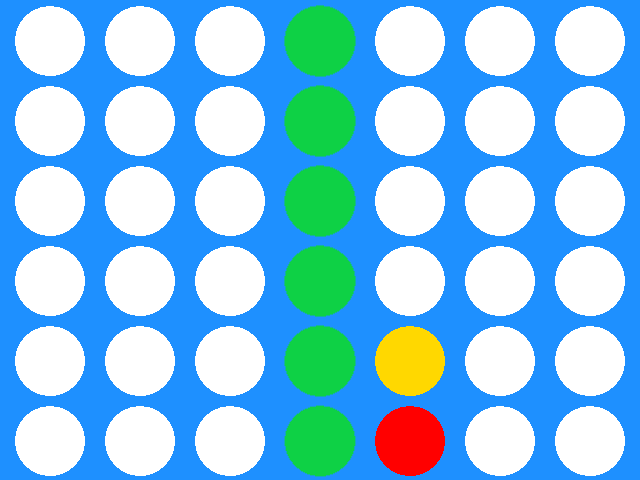
\includegraphics[width=0.6\textwidth]{images/connect_four_board_1.png}\\
                \end{column}
            \end{columns}
        \end{frame}

        \begin{frame}{Check for Four Connected Pieces}
            \LARGE
            Check Diagonals\\
            \begin{columns}
                \begin{column}{0.5\textwidth}
                    \centering
                    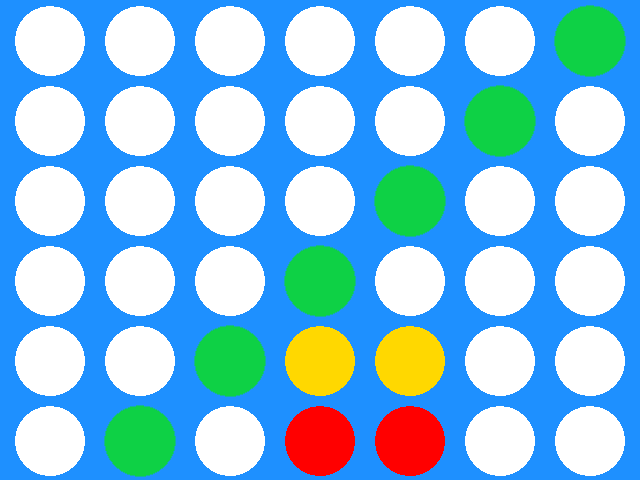
\includegraphics[width=0.6\textwidth]{images/connect_four_board_4.png}
                \end{column}
                \pause
                \begin{column}{0.5\textwidth}
                    \centering
                    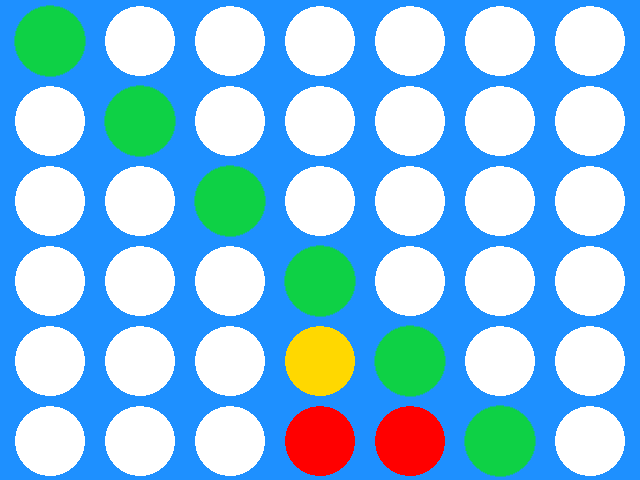
\includegraphics[width=0.6\textwidth]{images/connect_four_board_5.png}\\
                \end{column}
            \end{columns}
        \end{frame}

        \begin{frame}{Check for Four Connected Pieces}
            \LARGE
            You can use separate \texttt{for} Loops to go over row, column and diagonals.\\
            \pause
            You can create a counter to count connected pieces.
            \pause
            \begin{itemize}
                \item What happens to counter when we encounter a different piece?
            \end{itemize}
            \pause
            Counting only yellow pieces (\texttt{player\_piece}) is enough.\\
            \bigskip
            \begin{center}
                \Huge
                \textbf{HAVE FUN!}
            \end{center}
        \end{frame}

\end{document}